Por último se utiliza un índice hash sobre el campo `id' que genera Mongo a cada documento. Se eligió este campo ya que, al no poder elegir una clave compuesta, todos los campos generados por nosotros para las versiones de prueba se repetían demasiado (lo que hubiese generado hash parecidos, sino iguales).

\begin{figure}[h!]
 \centering
 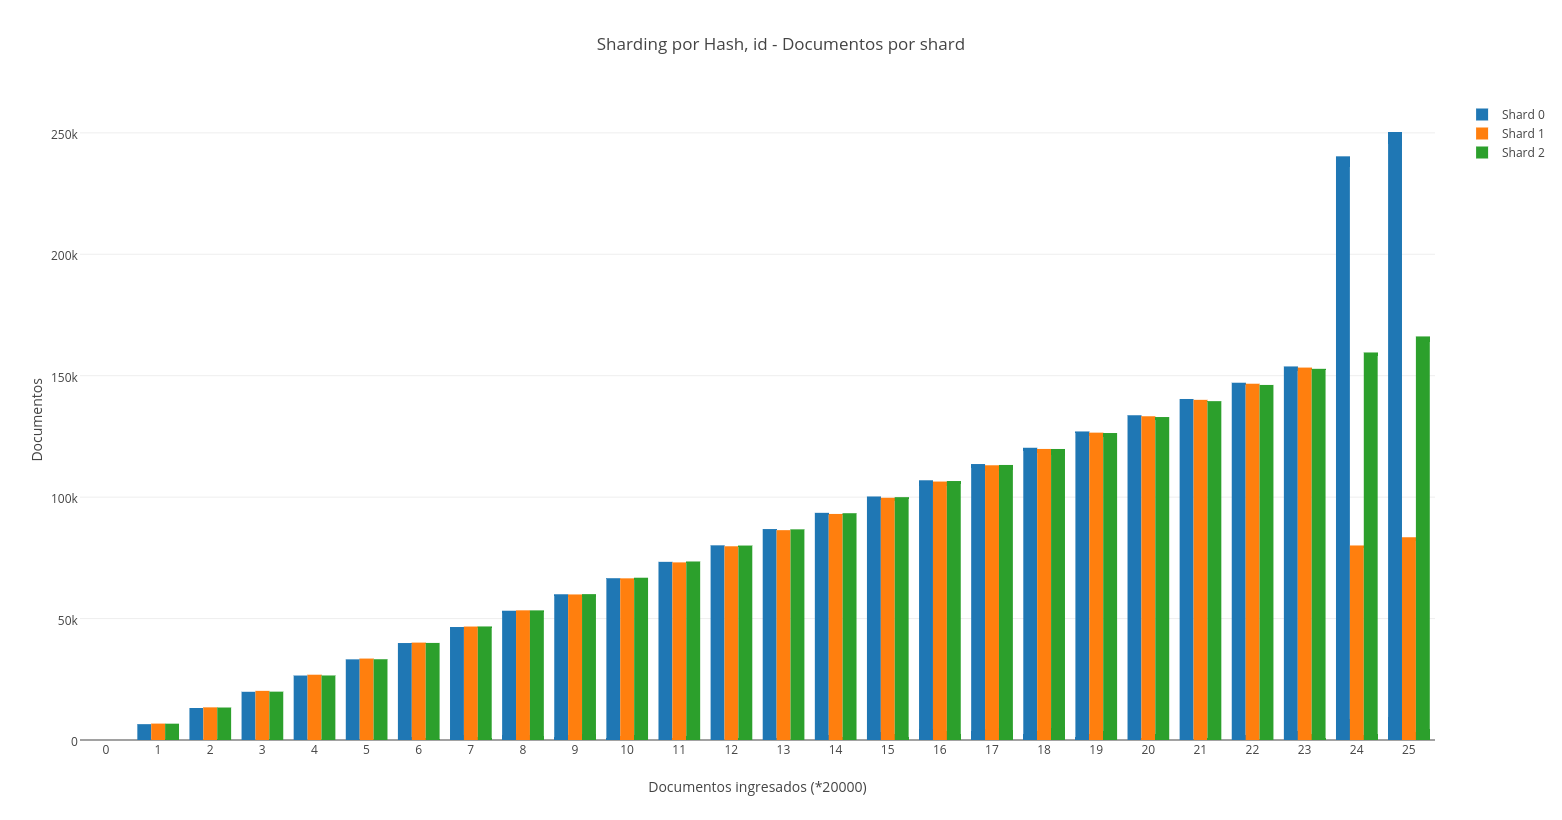
\includegraphics[scale=0.3]{./hash-documentos-por-shard.png}
 \caption{Documentos por shard}
\end{figure}

Vemos como se distribuyen uniformemente a medida que se ingresan datos. El cambio que se observa en la iteración 24 se puede deber a una mala elección de migración, esto, a medida que los datos crecen, se va corrigiendo. Ya que se espera, de un buen algoritmo de hash, una distribución uniforme.

\begin{figure}[h!]
 \centering
 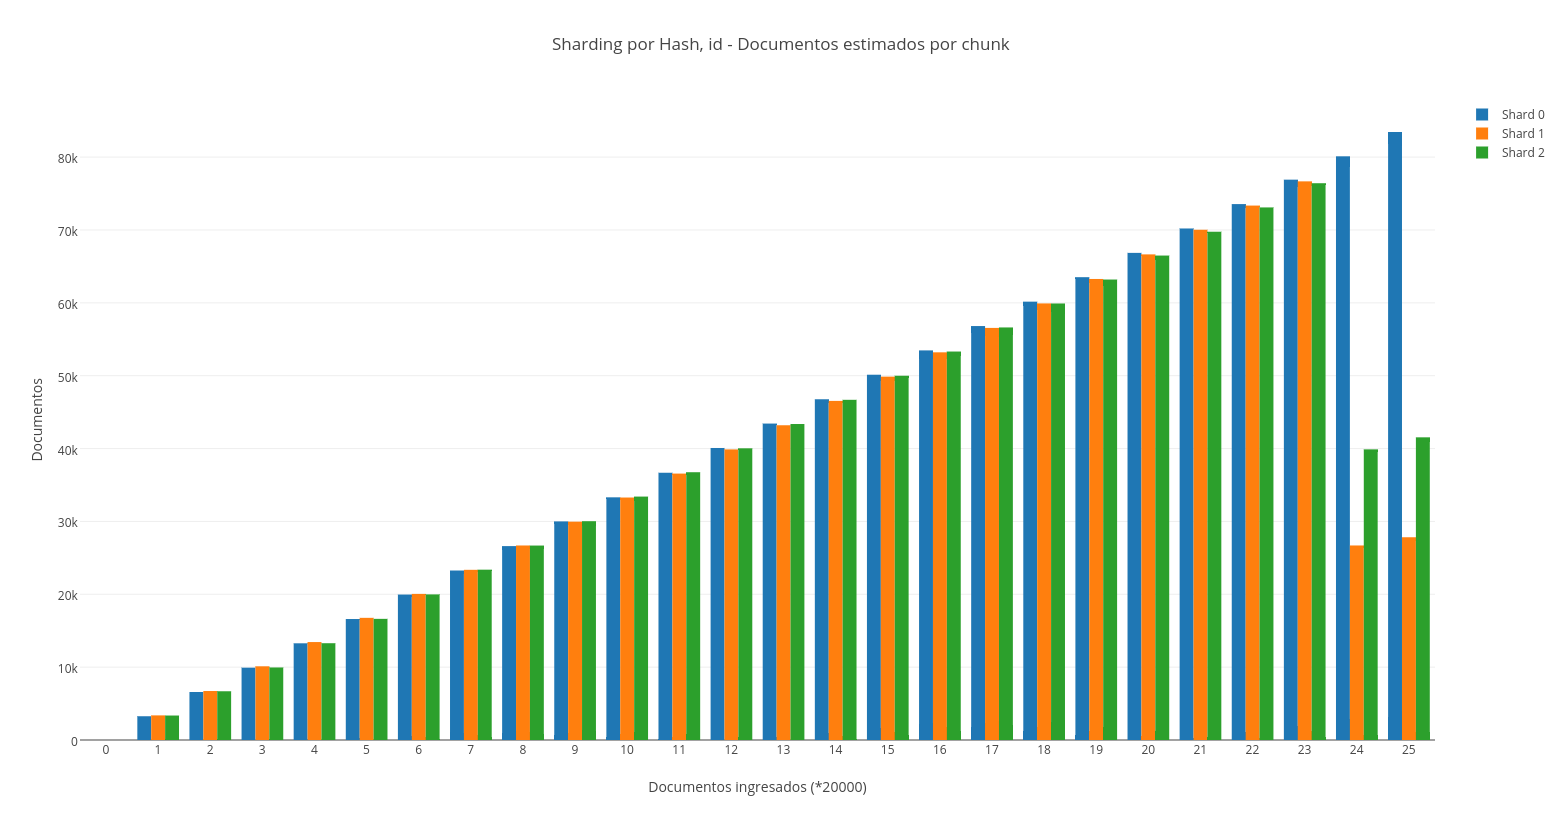
\includegraphics[scale=0.3]{./hash-documentos-estimados-por-chunk.png}
 \caption{Datos por chunk}
\end{figure}

Se observa que los chunks quedan desbalanceados en la iteración nro 24.
Quedando más cantidad de datos por chunk en el shard 0.\\

\begin{figure}[h!]
 \centering
 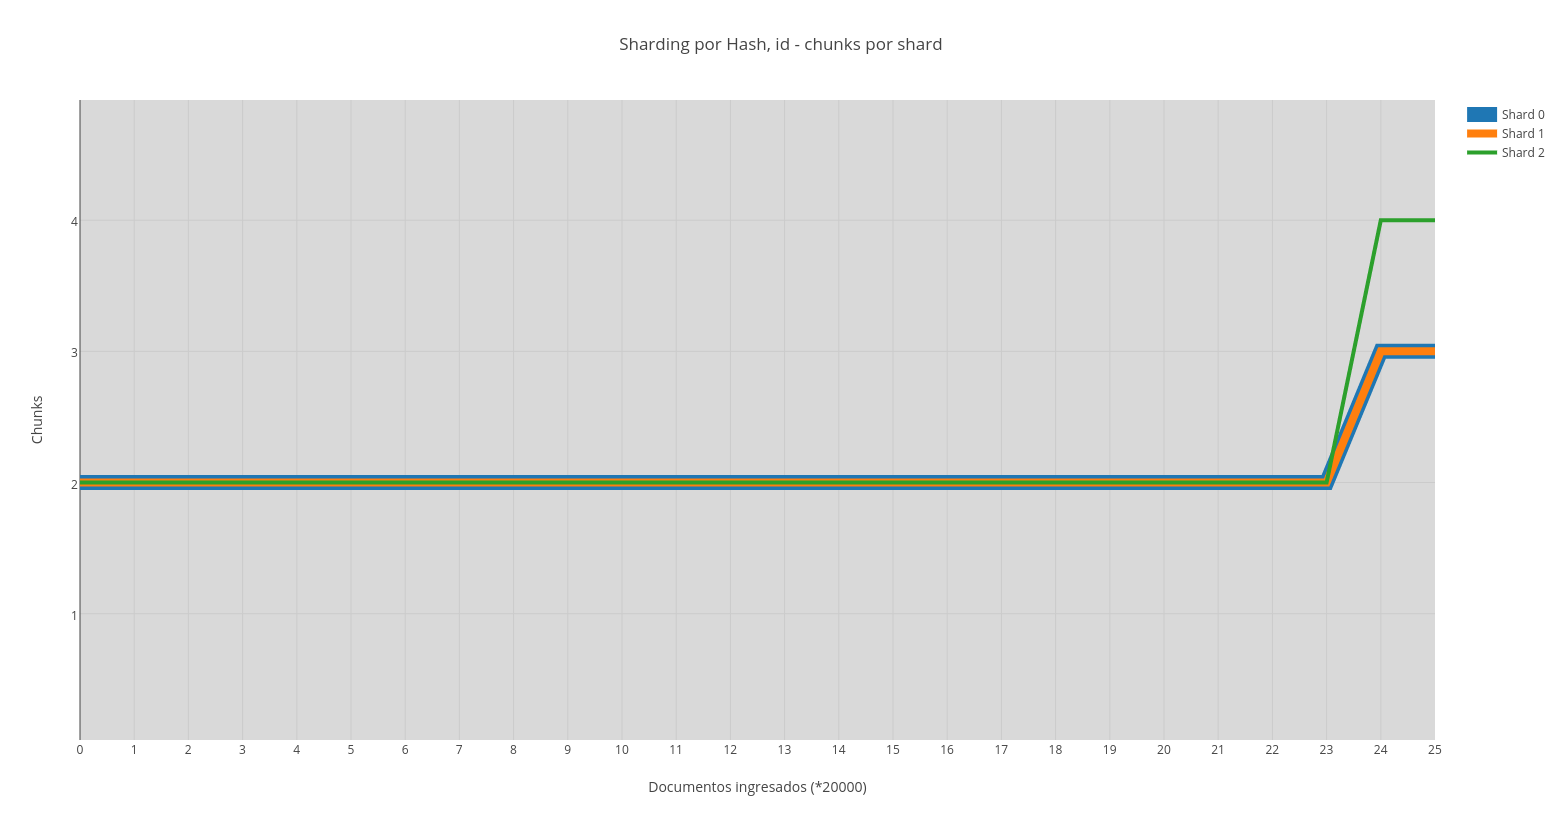
\includegraphics[scale=0.3]{./hash-cantidad-de-chunks-por-shard.png}
 \caption{Chunks por shard}
\end{figure}

Por último se muestra la cantidad de chunks por shard, permitiendo comparar mejor los gráficos anteriores.\\

Para observar mejor los gráficos se pueden acceder mediante los siguientes links a su representación online:
\begin{itemize}
 \item \href{https://plot.ly/~fzanollo/46/sharding-por-hash-id-documentos-por-shard/}{Documentos por shard}
 \item \href{https://plot.ly/~fzanollo/45/sharding-por-hash-id-documentos-estimados-por-chunk/}{Documentos estimados por chunk}
 \item \href{https://plot.ly/~fzanollo/44/sharding-por-hash-id-chunks-por-shard/}{Cantidad de chunks por shard}
\end{itemize}


